\section{Data Exchange}
Think of it like this: you want to send a message to your friend across the room. You could:
\begin{itemize}
    \item Flash a light on and off (optical)
    \item Tap on the table (mechanical vibrations)
    \item Speak out loud (sound waves)
\end{itemize}

In networks, we do something similar but with electricity, light, or radio waves. The key insight is that we're just changing something physical that the receiver can detect - like voltage going up and down, light getting brighter and dimmer, or radio waves shifting frequency.

\begin{importantblock}
    The process of converting bits into signals is called \textbf{modulation}, and the reverse process is called \textbf{demodulation}.
\end{importantblock}



\subsection{The Reality Check}

Here's where it gets interesting. In an electrical engineer's ideal world, digital signals would look like perfect rectangles - instant jumps from 0 to 1. But physics says that the harsh reality is that a perfect one is impossible to achieve in practice\footnote{Source -- \href{https://en.wikipedia.org/wiki/Square_wave_(waveform)\#Characteristics_of_imperfect_square_waves}{https://en.wikipedia.org/wiki/Square\_wave\_(waveform)}}, due to the lack of infinite bandwidth required to create it. Real signals are always more sinusoidal, with smooth transitions between high and low states.

\begin{figure}[h]
    \centering
    \includegraphics[width=.7\textwidth]{assets/osi/physical/waves.png}
    \caption{Theoretical waves}\label{fig:theoretical_waves}
\end{figure}

In practice, we use analog signals to transmit digital information. These analog signals are continuous and can take any value within a range. At the receiver, we need to convert these analog signals back to discrete digital values (\texttt{1} or \texttt{0}) through a process called \textbf{sampling and quantization}. The receiver samples the analog signal at specific time intervals and uses threshold levels to determine whether each sample represents a \texttt{1} or \texttt{0}.

Let's look at a simple example of a 1-bit ADC (Analog to Digital Converter) that converts a voltage level into a bit value:

% assets/osi/physical/adc_plot.png
\begin{figure}[h]
    \centering
    \includegraphics[width=.5\textwidth]{assets/osi/physical/adc_plot.png}
    \caption{Example of a 1-bit ADC converting voltage levels to bits}\label{fig:adc_plot}
\end{figure}

However, as you can probably guess, there are infinite ways for us to interpret this graph. It could correspond to \texttt{1010} or \texttt{1111000011110000} and so on. 
This is where clock signals come into play, which help us determine when to sample the signal and how to interpret it.

\subsection*{Let's talk timing $\star$}
Clocks or timing signals are present in all hardware communication. 

The idea is to ensure that both sender and receiver are synchronized in their understanding of when bits are being sent and received. 

As an analogy, think of a dance where both partners need to be in sync to perform the moves correctly. If one partner is out of sync, the dance will look awkward and may not work at all.


There are two main types of synchronization:
\begin{itemize}
    \item Both sender and receiver share a common clock signal (Figure~\ref{fig:clock_sync}) - Synchronous 
    \item Sender and receiver do not share a common clock, but use start and stop bits to indicate the beginning and end of a data frame - Asynchronous
\end{itemize}

\begin{figure}[h]
    \centering
    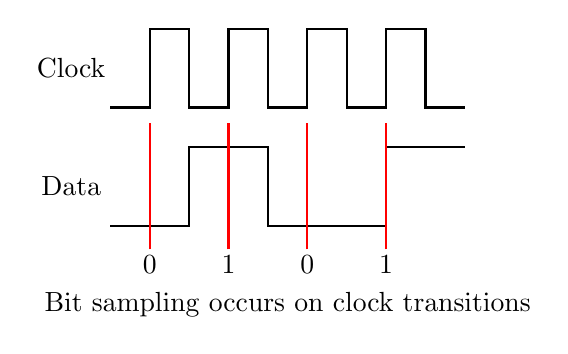
\begin{tikzpicture}
        % Clock signal
        \draw[thick] (0,2) -- (0.5,2) -- (0.5,3) -- (1,3) -- (1,2) -- (1.5,2) -- (1.5,3) -- (2,3) -- (2,2) -- (2.5,2) -- (2.5,3) -- (3,3) -- (3,2) -- (3.5,2) -- (3.5,3) -- (4,3) -- (4,2) -- (4.5,2);
        \node at (-0.5,2.5) {Clock};
        
        % Data signal
        \draw[thick] (0,0.5) -- (1,0.5) -- (1,1.5) -- (2,1.5) -- (2,0.5) -- (3.5,0.5) -- (3.5,1.5) -- (4.5,1.5);
        \node at (-0.5,1) {Data};
        
        % Sampling points
        \foreach \x in {0.5,1.5,2.5,3.5}
            \draw[red,thick] (\x,0.2) -- (\x,1.8);
        
        % Bit values
        \node at (0.5,0) {0};
        \node at (1.5,0) {1};
        \node at (2.5,0) {0};
        \node at (3.5,0) {1};
        
        % Labels
        \node at (2.25,-0.5) {Bit sampling occurs on clock transitions};
    \end{tikzpicture}
    \caption{Example rising edge clock synchronization}\label{fig:clock_sync}
\end{figure}

\vfill
In asynchronous serial\footnote{
    Serial - \textit{one after another} - communication, data is sent one bit at a time over a single channel. This is in contrast to parallel communication. More on that in the Operating Systems course.
} communication, data is organized into discrete blocks called code words of fixed length - usually bytes or ASCII characters (\texttt{char}s are $2^8 = 256$ bits, i.e. a byte). Each code word is framed by:

\begin{figure}[h]
    \centering
    \input{assets/diagrams/physical.latex}
    \caption{Async serial frame structure}\label{fig:async_frame}
\end{figure}

This approach, specifically in the form that we refer to in the figure, is \textbf{character-oriented}.
\vfill
\section{Modulation and Encoding}\label{sec:modulation}
As mentioned earlier, modulation is the process of converting digital data into analog signals for transmission over a physical medium.

\begin{figure}[h]
    \centering
    \includegraphics[width=\textwidth]{assets/osi/physical/signals/modulation.png}
    \caption{Modulation techniques}\label{fig:modulation_techniques}
\end{figure}

\subsection{The basics}
We'll start with something most people are familiar with, as it is used in consumer radios! The ones you listen to in your car or at home.

Amplitude Modulation (AM) and Frequency Modulation (FM) are two very common modulations used in radio broadcasting, where we are used to hearing music and news. We are used to tuning our radios to a specific frequency ($\approx$ 80-100 MHz for FM and usually way lower for AM) to listen to our favorite stations.

There's also Phase Modulation (PM), where the phase of the carrier wave is varied according to the input signal.
\begin{figure}[h]
    \centering
    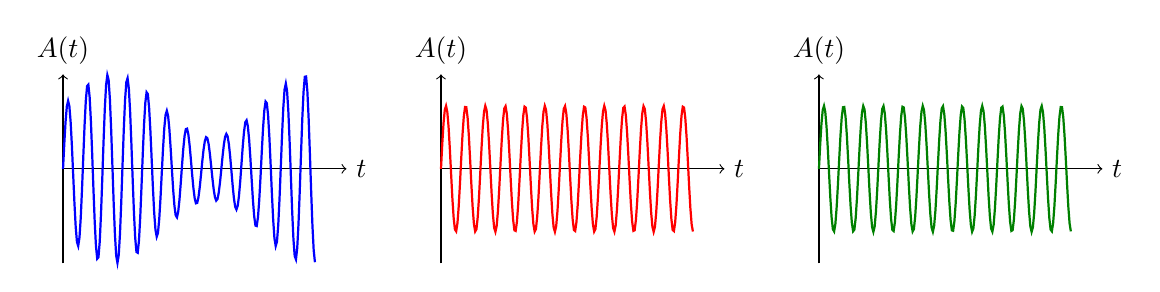
\begin{tikzpicture}[scale=0.8]
        % AM Signal
        \begin{scope}[shift={(0,0)}]
            \draw[->] (0,0) -- (4.5,0) node[right] {$t$};
            \draw[->] (0,-1.5) -- (0,1.5) node[above] {$A(t)$};
            \draw[domain=0:4,samples=200,thick,blue] plot (\x,{(1+0.5*sin(2*\x r))*sin(20*\x r)});
        \end{scope}
        
        % FM Signal
        \begin{scope}[shift={(6,0)}]
            \draw[->] (0,0) -- (4.5,0) node[right] {$t$};
            \draw[->] (0,-1.5) -- (0,1.5) node[above] {$A(t)$};
            \draw[domain=0:4,samples=200,thick,red] plot (\x,{sin(20*\x r + 2*sin(2*\x r))});
        \end{scope}
        
        % PM Signal
        \begin{scope}[shift={(12,0)}]
            \draw[->] (0,0) -- (4.5,0) node[right] {$t$};
            \draw[->] (0,-1.5) -- (0,1.5) node[above] {$A(t)$};
            \draw[domain=0:4,samples=200,thick,green!50!black] plot (\x,{sin(20*\x r + 0.5*sin(2*\x r))});
        \end{scope}
    \end{tikzpicture}
    \caption{Graphical representation of \textcolor{blue}{AM}, \textcolor{red}{FM}, and \textcolor{green!50!black}{PM} signals.}\label{fig:modulation_math}
\end{figure}


But wait, we have only heard voices and music, not bits! How does that work?

The answer lies in \textbf{digital modulation}! While AM and FM were originally designed for analog voice transmission, the same radio frequencies can carry digital data using techniques like DMR, WSPR, and many, many more.
These digital protocols use discrete changes in amplitude, frequency, or phase to represent bits.

For example, in WSPR, a \texttt{1} might be represented by a short burst of a specific frequency, while a \texttt{0} might be represented by silence or a different frequency - this is called \textbf{frequency-shift keying (FSK)}.


\begin{figure}[h]
    \centering
    \begin{subfigure}[b]{0.2\textwidth}
        \centering
        \includegraphics[width=\textwidth]{assets/osi/physical/signals/am_voice.png}
        \caption{AM Voice Signal}
        \label{fig:am_voice}
    \end{subfigure}
    \hspace{1em}
    \begin{subfigure}[b]{0.2\textwidth}
        \centering
        \includegraphics[width=\textwidth]{assets/osi/physical/signals/fm_voice.png}
        \caption{FM Voice Signal}
        \label{fig:fm_voice}
    \end{subfigure}
    \hspace{1em}
    \begin{subfigure}[b]{0.2\textwidth}
        \centering
        \includegraphics[width=\textwidth]{assets/osi/physical/signals/dmr.png}
        \caption{DMR Digital Signal}
        \label{fig:dmr_digital}
    \end{subfigure}
    \hspace{1em}
    \begin{subfigure}[b]{0.2\textwidth}
        \centering
        \includegraphics[width=\textwidth]{assets/osi/physical/signals/wspr.png}
        \caption{WSPR Digital Protocol}
        \label{fig:wspr_digital}
    \end{subfigure}
    
    \caption{Comparison of analog voice signals (a, b) vs digital signals (c, d) in the radio spectrum. Sourced from sigidwiki.com}
    \label{fig:analog_vs_digital_signals}
\end{figure}

\newpage
For digital data, modulation becomes synonymous with \textbf{keying}, where we use changes in the signal to represent bits.

\begin{itemize}
    \item Amplitude Shift Keying (ASK) -  A higher amplitude might represent a \texttt{1}, while a lower amplitude represents a \texttt{0}.
    \item Frequency Shift Keying (FSK) - Different frequencies represent different bits.
    \item Phase Shift Keying (PSK) - A phase shift might represent a \texttt{1}, while no shift represents a \texttt{0}.
\end{itemize}
\begin{figure}[h]
    \centering
    \includegraphics[width=0.45\textwidth]{assets/osi/physical/signals/sk.png}
    \caption{Keying techniques: ASK, FSK, PSK}\label{fig:keying_techniques}
\end{figure}

\subsection{Quadrature Amplitude Modulation (QAM)}
What if we could send multiple bits at once? That's where QAM comes in, which is a combination of both amplitude and phase modulation.

`Quadrature' just means we're using two waves that are perfectly out of sync - 90 degrees out of phase, to be exact (quad = four, so in a circle $\frac{360}{4} = 90$).

\subsubsection{Complex Numbers and QAM $\star$}
To completely understand QAM, we will need to quickly refresh our knowledge of complex numbers. If you are not familiar with them, I recommend reading the \href{https://en.wikipedia.org/wiki/Complex_number}{Wikipedia article}. 

QAM transmits data using two independent carrier waves at the same frequency but shifted 90 degrees apart in phase - called `in-phase' ($I$) and `quadrature' ($Q$) components. This orthogonal\footnote{
    Remember orthogonality! It's a cheat code in signal processing! It means the two signals don't interfere with each other and can be separated at the receiver.
} relationship means the two signals don't interfere with each other and can be separated at the receiver.

Complex numbers provide an elegant mathematical framework for this because:
\begin{itemize}
    \item The real part represents the in-phase ($I$) component
    \item The imaginary part represents the quadrature ($Q$) component  
    \item A 90-degree phase shift is equivalent to multiplication by $i$ (since $e^{i\pi/2} = i$)
    \item Both amplitude and phase information are present in a single complex number $z = $I$ + iQ$
\end{itemize}

\begin{figure}[h]
    \centering
    \includegraphics[width=0.5\textwidth]{assets/diagrams/iq.png}
\end{figure}

This is why we call it "Quadrature" - it literally refers to the four quadrants of this complex plane, where signals can point in any direction to encode different bit combinations.

\subsubsection{What does the number mean?}
When working with QAM, we will often see terms like 16-QAM, 64-QAM, etc. These numbers refer to the number of distinct symbols that can be transmitted. For example:
\begin{itemize}
    \item 16-QAM can transmit 16 different symbols, each representing 4 bits
    \item 64-QAM can transmit 64 different symbols, each representing 6 bits
    \item 256-QAM can transmit 256 different symbols, each representing 8 bits
\end{itemize}

You may notice the pattern in the above examples - the number of bits per symbol is given by $\log_2(N)$, where $N$ is the number of symbols.

This will immediately make sense in the next section.
\subsection{Constellation Diagrams}
A constellation diagram is a graphical representation of digital modulation schemes. Each point in the diagram represents a unique symbol that can be transmitted, with its position determined by the signal's characteristics. That's nerdspeak for points on a graph.

\begin{figure}[h]
    \centering
    \includegraphics[width=0.5\textwidth]{assets/osi/physical/signals/qam.png}
    \caption{Example of a 16-QAM \textbf{cartesian} constellation diagram}\label{fig:qam_constellation}
\end{figure}


For QAM, the position is determined by the in-phase ($I$) and quadrature ($Q$) components (x, y coordinates). For other modulation schemes:
\begin{itemize}
    \item In PSK, points are arranged in a circle, with phase determining the angular position
    \item In ASK, points are arranged on a line, with amplitude determining the position
\end{itemize}

\begin{importantblock}
    You can probably see that ASK+PSK is QAM, since, by definition, it combines both amplitude and phase modulation.
\end{importantblock}

In any constellation diagram, each point represents a unique combination of signal parameters. The distance between points determines the minimum distance between symbols, which affects the error rate in transmission. The more points we have, the more bits we can transmit per symbol, but the closer they are together, the easier it is to confuse them at the receiver.

There are different ways to visualize these diagrams, for example, when treating ASK+PSK (component-wise, instead as a single complex number), we can plot the amplitude and phase separately as concentric circles with points scattered accross their respective circumferences. This is called a \textbf{polar constellation diagram}.

Let's look at an example of a 4-QAM (ASK+PSK) constellation diagram.
\begin{figure}[h]
    \centering
    \includegraphics[width=0.5\textwidth]{assets/osi/physical/signals/ask+psk.png}
    \caption{Example of a 4-QAM \textbf{polar constellation diagram}}\label{fig:ask_psk_constellation}
\end{figure}

Now, say we want to encode the binary string \texttt{00101101}. We can map it to the 4-QAM constellation diagram as follows:

\begin{itemize}
    \item \texttt{00} maps to the first point on the left of outer circle
    \item \texttt{10} maps to the second point on the top of inner circle
    \item \texttt{11} maps to the third point on the right of outer circle
    \item \texttt{01} maps to the fourth point on the bottom of inner circle
\end{itemize}

Resulting in the following mapping:
\begin{figure}[h]
    \centering
    \includegraphics[width=0.5\textwidth]{assets/osi/physical/signals/ask+psk_filled.png}
    \caption{Example of a 4-QAM constellation diagram with bits mapped to points}\
    \label{fig:ask_psk_filled_constellation}
\end{figure}

Again, this mapping is arbitrary, and we can choose any mapping we want, as long as the receiver knows how to interpret it (which, hypothetically, it always does).

Since we have both amplitude and phase information for each constellation point, we can plot the actual time-domain waveforms that correspond to each symbol - showing how the signal actually looks during transmission!

Let's do so for this example.

\subsubsection{Time-Domain Waveforms}
Each constellation point can be expressed as a complex number with amplitude $A$ and phase $\phi$:
$$s(t) = A \cos(2\pi f_c t + \phi)$$

where $f_c$ is the carrier frequency. For our 4-QAM example with bit string \texttt{00101101}, the complete transmitted signal looks like:

\begin{figure}[h]
    \centering
    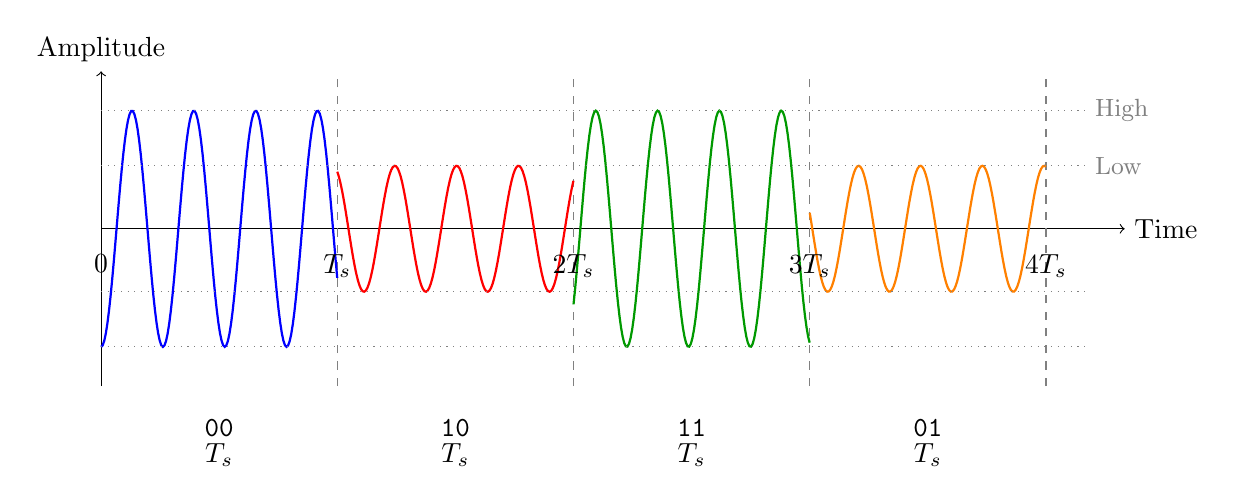
\begin{tikzpicture}[scale=1]
        % Main axes
        \draw[->] (0,0) -- (13,0) node[right] {Time};
        \draw[->] (0,-2) -- (0,2) node[above] {Amplitude};
        
        % Symbol boundaries (vertical dashed lines)
        \foreach \x in {3,6,9,12} {
            \draw[dashed, gray] (\x,-2) -- (\x,2);
        }
        
        % Symbol period labels
        \node[below] at (1.5,-2.3) {\texttt{00}};
        \node[below] at (4.5,-2.3) {\texttt{10}};
        \node[below] at (7.5,-2.3) {\texttt{11}};
        \node[below] at (10.5,-2.3) {\texttt{01}};
        
        % Symbol period markers
        \node[below] at (1.5,-2.6) {$T_s$};
        \node[below] at (4.5,-2.6) {$T_s$};
        \node[below] at (7.5,-2.6) {$T_s$};
        \node[below] at (10.5,-2.6) {$T_s$};
        
        % Complete waveform
        % Symbol 1: 00 (High amp, 180° phase) - inverted high amplitude cosine
        \draw[domain=0:3,samples=150,thick,blue] plot (\x,{1.5*cos(8*\x r + 180)});
        
        % Symbol 2: 10 (Low amp, 90° phase) - low amplitude sine  
        \draw[domain=3:6,samples=150,thick,red] plot (\x,{0.8*cos(8*\x r + 90)});
        
        % Symbol 3: 11 (High amp, 0° phase) - normal high amplitude cosine
        \draw[domain=6:9,samples=150,thick,green!60!black] plot (\x,{1.5*cos(8*\x r)});
        
        % Symbol 4: 01 (Low amp, 270° phase) - low amplitude negative sine
        \draw[domain=9:12,samples=150,thick,orange] plot (\x,{0.8*cos(8*\x r + 270)});
        
        % Amplitude level indicators
        \draw[dotted, gray] (0,1.5) -- (12.5,1.5) node[right] {\small High};
        \draw[dotted, gray] (0,0.8) -- (12.5,0.8) node[right] {\small Low};
        \draw[dotted, gray] (0,-0.8) -- (12.5,-0.8);
        \draw[dotted, gray] (0,-1.5) -- (12.5,-1.5);
        
        % Time axis labels
        \node[below] at (0,-0.2) {0};
        \node[below] at (3,-0.2) {$T_s$};
        \node[below] at (6,-0.2) {$2T_s$};
        \node[below] at (9,-0.2) {$3T_s$};
        \node[below] at (12,-0.2) {$4T_s$};
    \end{tikzpicture}
    \caption{Complete time-domain signal for bit string \texttt{00101101} using 4-QAM modulation. Each symbol period $T_s$ contains one constellation point with its specific amplitude and phase.}
    \label{fig:qam_complete_waveform}
\end{figure}

\begin{tipblock}
    In practice, these individual symbol waveforms are concatenated to form the complete transmitted signal. The receiver uses matched filtering and decision algorithms to determine which constellation point was transmitted by analyzing the received waveform during each symbol period.
\end{tipblock}